\documentclass[fleqn, a4paper]{report}
\usepackage[top=1.5in,bottom=1.5in,left=1.15in,right=1.15in]{geometry}
\usepackage{graphicx}
\usepackage{tikz}
\usetikzlibrary{automata, positioning, arrows}
\usepackage[export]{adjustbox}
\usepackage{float}
\usepackage{amsmath}
\usepackage{pgfplots}
\usepackage{subfig}
\pgfplotsset{compat=1.15}
\usepackage[utf8]{inputenc}
\usepackage{hyperref}
\hypersetup{
    colorlinks=true,
    linkcolor=blue,
    filecolor=magenta,      
    urlcolor=cyan,
}

\title{EE463 Static Power Conversion I 
-Simulation Project I}
\author{Nail Tosun, Yusuf Selim Karataş}
\date{November 2018}

\usepackage{natbib}
\usepackage{graphicx}

\begin{document}


\maketitle

\section*{Introduction}
In this simulation project, we investigated single phase and three phase diode rectifier topologies. The effects of different sample time on Simulink discussed Q1. The effects of load configurations on output voltage waveform, average voltage and THD of line current proposed first part of Q2. Selection of diode and rectifier module be explained part 2. Selection of proper dc bus capacitor with given performance requirement explained part 3. The effect of line inductance on output voltage waveform, source current is discussed part 4. At final part of Q2 we draw voltage waveform at PCC and saw the effect of nonlinear load. 
\section*{Abbreviations}
\begin{table}[H]
\begin{tabular}{ll}
\textbf{THD} & Total Harmonic Distortion \\
\textbf{Qx}  & x'th question \\
\textbf{PCC} & Point of Common Coupling \\
\textbf{l-l} & Line to Line 
\end{tabular}
\end{table}
\section*{Question 1}
In this question we investigated the effects of different discrete step sizes on simulation in Simulink environment. Firstly we built single phase diode rectifier which connected through Turkish electrical grid ($400 V_{l-l}$ ). We connected 3 470 $\mu$F capacitors to make output voltage smoother and this will not have any effect on the resolution of waveforms. 
\begin{figure}[H]
  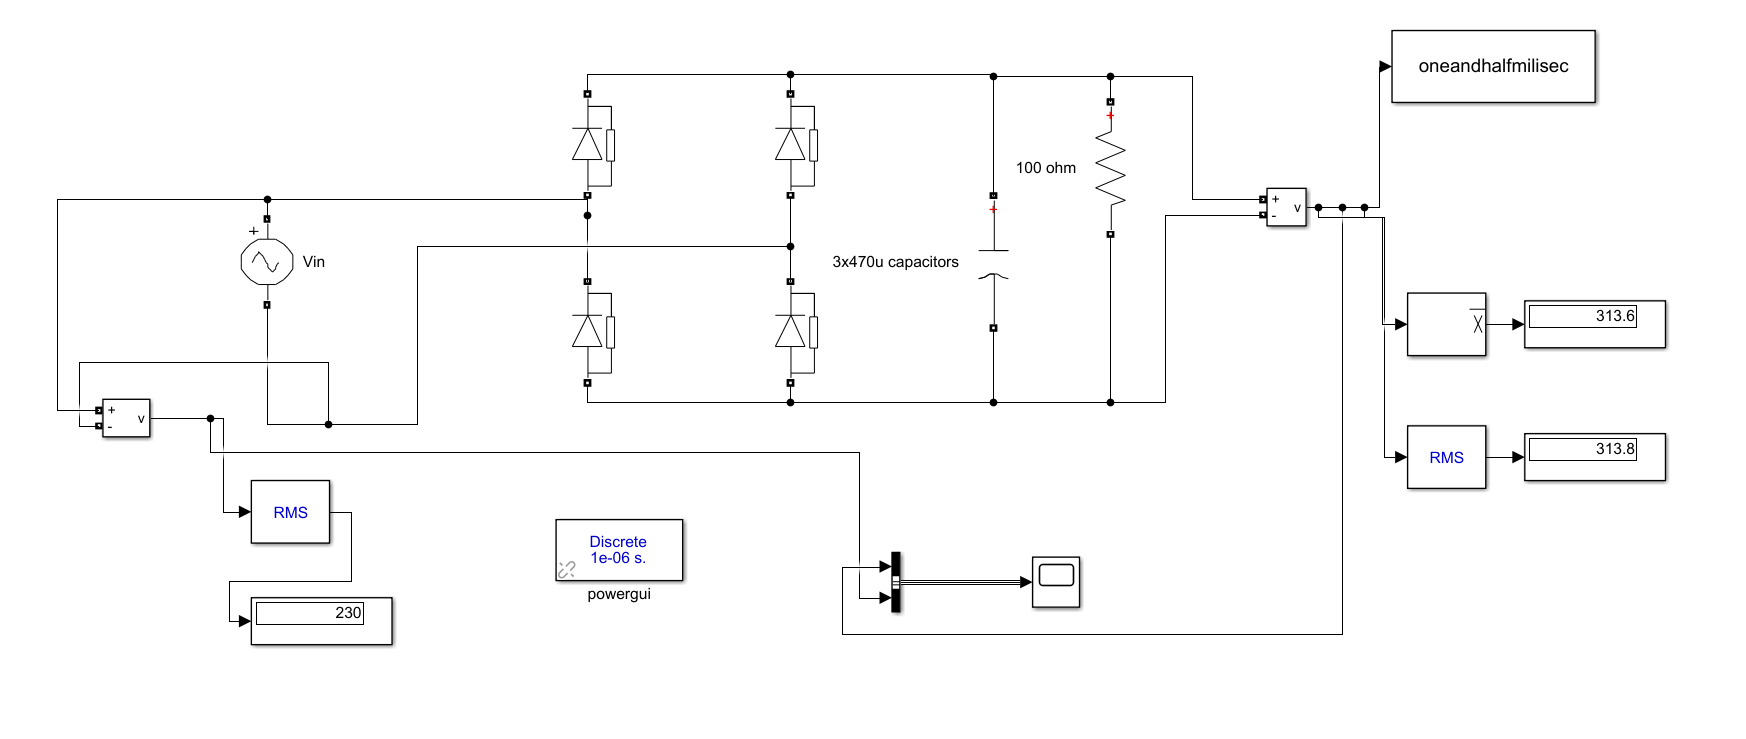
\includegraphics[width=\linewidth]{question-1-simulink-model.PNG}
  \caption{Simulink model of single phase diode rectifier}
  \label{fig:simulink2}
\end{figure}
\begin{figure}[H]
  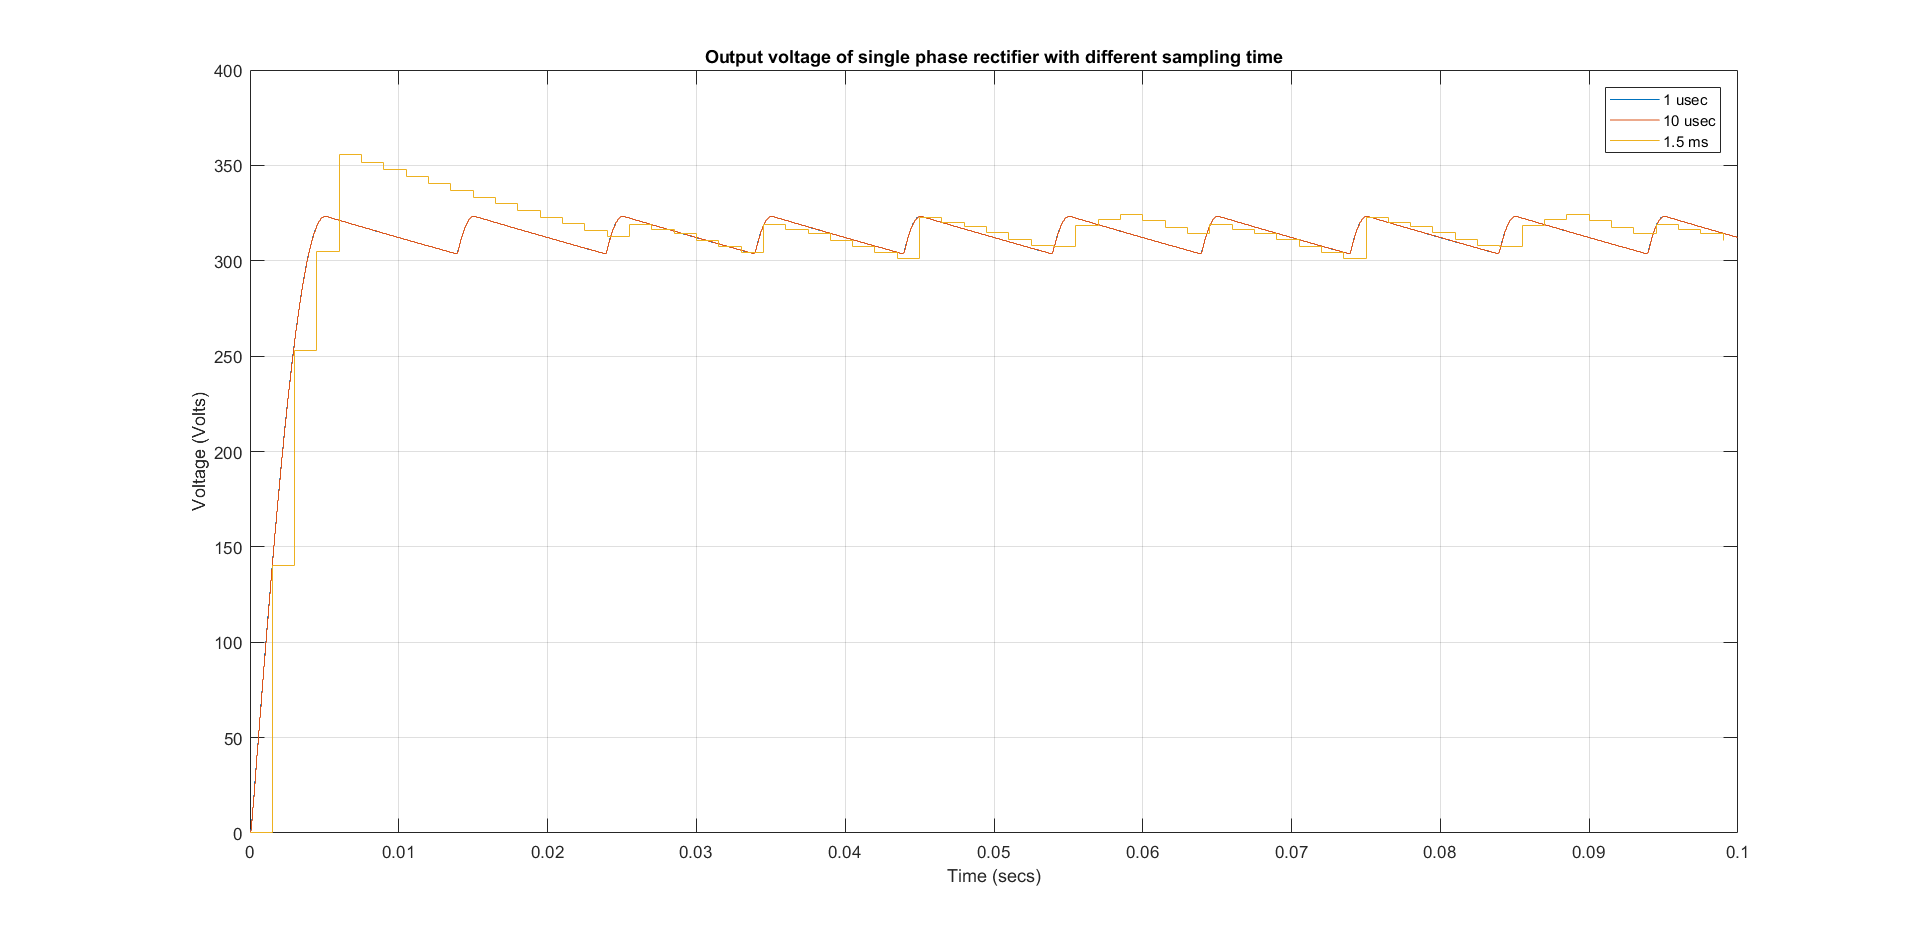
\includegraphics[width=\linewidth]{Q1_plots_different_samplings.png}
  \caption{Transients of voltage waveforms under various sampling frequencies}
  \label{fig:simulink2}
\end{figure}
\begin{figure}[H]
  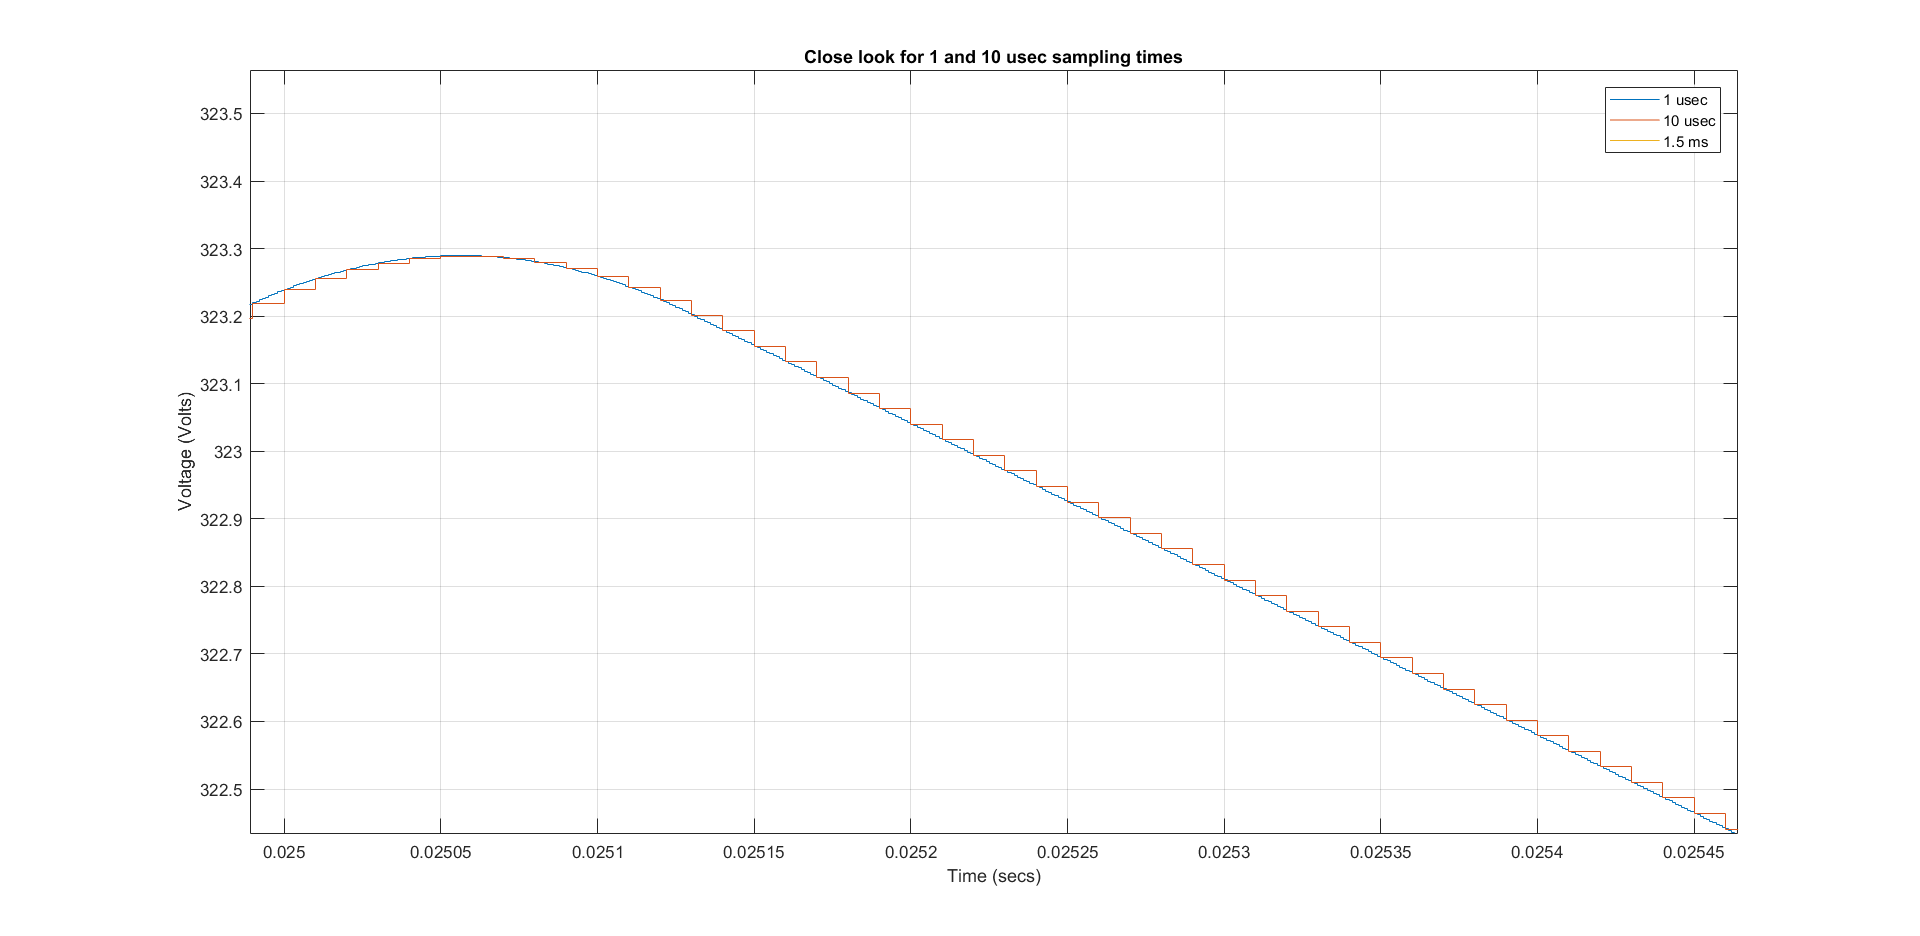
\includegraphics[width=\linewidth]{closer-look.png}
  \caption{Closer look for 1usec and 10usec to see transients}
  \label{fig:simulink2}
\end{figure}
We observed that, with large step size we lose some transients (especially at 1.5ms) but simulation time reduce since it is computationally inexpensive. With 50 Hz input signal there is no such difference between 1 $\mu$sec and 10 $\mu$sec however 1 $\mu$sec has 10 times more computational work. Therefore an engineer should do trade-off between resolution and computation time according to his or her requirements.  
\section*{Question 2}
We built single phase rectifier in Simulink environment, using full-wave topology. 
\subsection*{Part 1}
Then we simulate the system different with different load configurations namely;
\begin{itemize}
	\item R = 25 ohm
	\item R = 25 ohm L = 10 mH
	\item R = 25 ohm L = 1 H
\end{itemize}
\begin{figure}[H]%
    \centering
    \subfloat[R=25 ohm]{{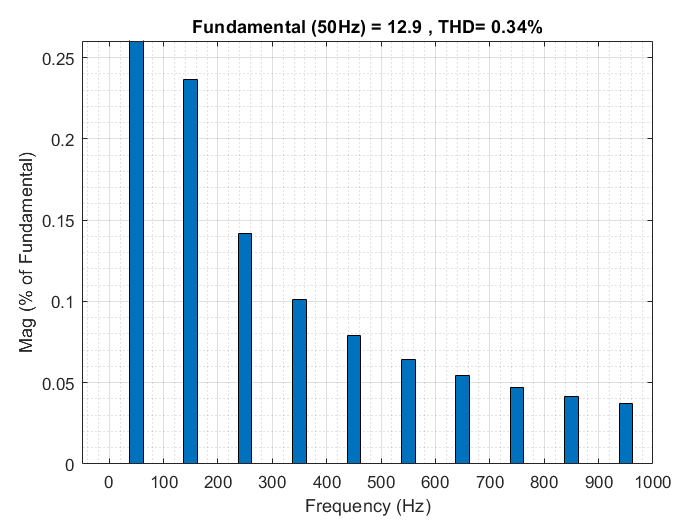
\includegraphics[width=5cm]{thd_resistive.png}}}%
    \qquad
    \subfloat[R=25 ohm L = 10 mH]{{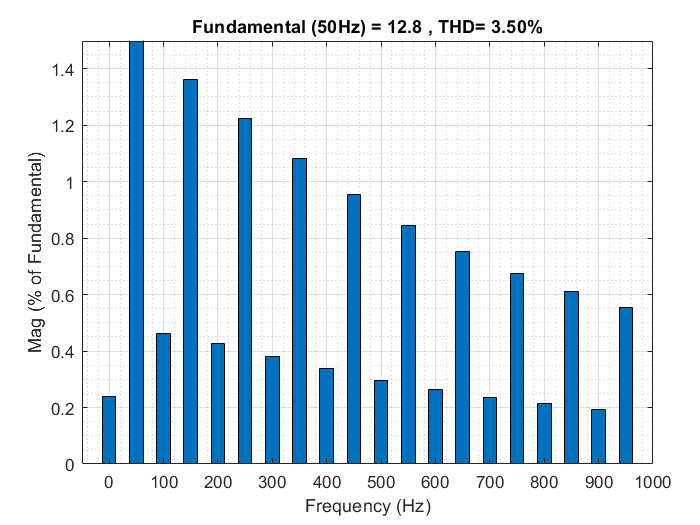
\includegraphics[width=5cm]{tenmh.png} }}%
    \qquad
    \subfloat[R=25 ohm L = 1 H]{{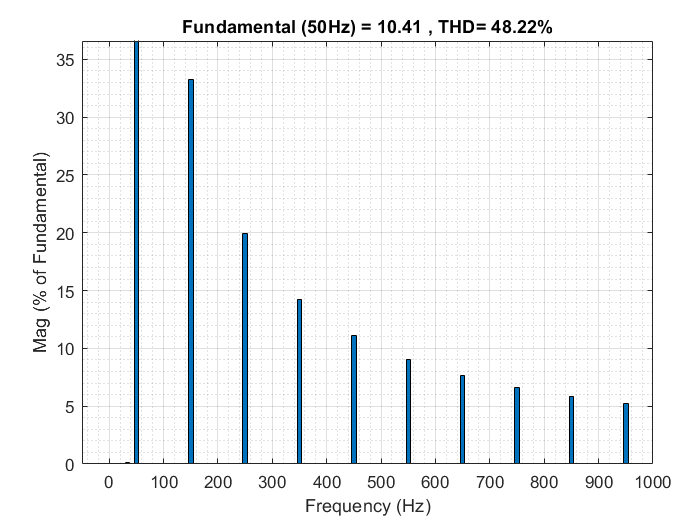
\includegraphics[width=5cm]{onehenry.png} }}%
    \caption{FFT analysis with different load configrations}%
    \label{fig:example}%
\end{figure}

\begin{table}[H]
\centering
\begin{tabular}{ll}
                      & THD      \\
R = 25 ohm            & \% 0.34  \\
R = 25 ohm L  = 10 mH & \% 3.5   \\
R = 25 ohm L = 1 H    & \% 48.22
\end{tabular}
\caption{THD with different load configurations}
\end{table} 

With only resistive load line current is sinusoidal therefore THD is very low. With increasing L load behave like current source therefore line current waveform starts to disrupt. At high inductance like 1 H the inductor behave like \textbf{ideal current source} and the line current become square wave (THD becomes \% 48).  If inductance goes to infinity, it acts as ideal current source.


\begin{figure}[H]
  \includegraphics[width=\linewidth]{output_waveforms21.png}
  \caption{Output Voltage Waveforms under different load configurations}
  \label{fig:simulink2}
\end{figure}

\begin{table}[H]
\centering
\begin{tabular}{ll}
Load configurations    & Average Output Voltage \\
R = 25 ohm            & 204.9 V                \\
R = 25 ohm L  = 10 mH & 204.9 V                \\
R = 25 ohm L = 1 H    & 204.9 V               
\end{tabular}
\end{table}

As can be seen in Figure 5, when commutation ignored neither voltage waveforms nor average voltage changed when inductance has been increased. But when inductance of the load increases, despite of how quick voltage changes, current can not accompany at the same rate, and becomes smoother.

\subsection*{Part 2}
We choose MUR1540G with 15 A average current capability and 400 V peak repetitive reverse voltage. We make worst scenario for maximum current and peak reverse voltage. 
When load is 25 Ohm and 25 Ohm 1mH, maximum current emerges as 9.147 Amperes and our single diodes ara capable of 15 Amperes, so in terms of current capacity, selected diode will be more than enough. Also they have 1.25 V voltage drop when delivering 15A at the output. In this conditions, voltage drop on 2 conducting diodes will maximum be arround 2 Volts which is less than 1% of the input voltage. For 50 Hz grid, diodes have 10ms to revocer themselves and 60 ns which is time required MUR1540GOS-ND to recover itself is pretty good number. 

\begin{table}[H]
\centering
\begin{tabular}{ll}

Reverse Voltage                   & 400 V               \\
Current Average Reectified        & 15 A                \\
Voltage Forward                   & 1.25 V @ 15A        \\
Reverse Recovery Time             & 60 ns       	\\
Current Reverse Leakage           & 10 $\mu$A  @ 400V         
\end{tabular}
\caption{Electrical parameters of MUR1540GOS-ND}
\end{table}
Related link of the product is given below.

\url {https://www.digikey.com/product-detail/en/on-semiconductor/MUR1540G/MUR1540GOS-ND/919901}

As a rectifier module, we have decided upon using GBU1510TB which has 1655-1846-ND Digikey number. This module can withstand to 1100 V which is pretty much than single diode. Both have same current capacity but diode module has slightly less voltage drop under rated amper. Also it can be cheap as 0.4 US Dollars. When we compare single diode with diode rectifier module, we can easily see that, while rectifier module has better capabilities, it is much more cheaper than the four piece single diode module. Using rectifier module is more economical.

\begin{table}[H]
\centering
\begin{tabular}{ll}

Reverse Voltage                   & 1100 V               \\
Current Average Reectified        & 15 A                \\
Voltage Forward                   & 1.1 V @ 15A        \\
Current Reverse Leakage           & 5 $\mu$A  @ 1000V         
\end{tabular}
\caption{Electrical parameters of 1655-1846-ND}
\end{table}
Related link of the product is given below.

\url {https://www.digikey.com/product-detail/en/smc-diode-solutions/GBU1510TB/1655-1846-ND/7244874}

\subsection*{Part 3}
We added $560 \mu F $ electrolytic capacitor (565-2780-ND) decrease output voltage ripple. Some electrical parameters are given as table 1:
\begin{table}[H]
\centering
\begin{tabular}{ll}
Electrical Parameters & Average output voltage \\
Rated Voltage         & 400 V                  \\
Tolerance             & ± \%20                 \\
Capacitance           & 560 uF                 \\
Life-Time             & 2000 Hrs @ 85°C        \\
Ripple Current        & 2.69A @ 120Hz         
\end{tabular}
\caption{Electrical parameters of 565-2780-ND}

\end{table}
Related link of the product is given below.

\url{https://www.digikey.com/product-detail/en/united-chemi-con/ESMQ401VSN561MR45S/565-2780-ND/757993}

We choose $560 \mu F $ electrolytic capacitors since aluminum electrolytic capacitors have high tolerance. Although $470 \mu F $ capacitors meet out performance requirements we think worst case scenario (-\%20 ) as well. Our output waveforms are;
\begin{figure}[H]
  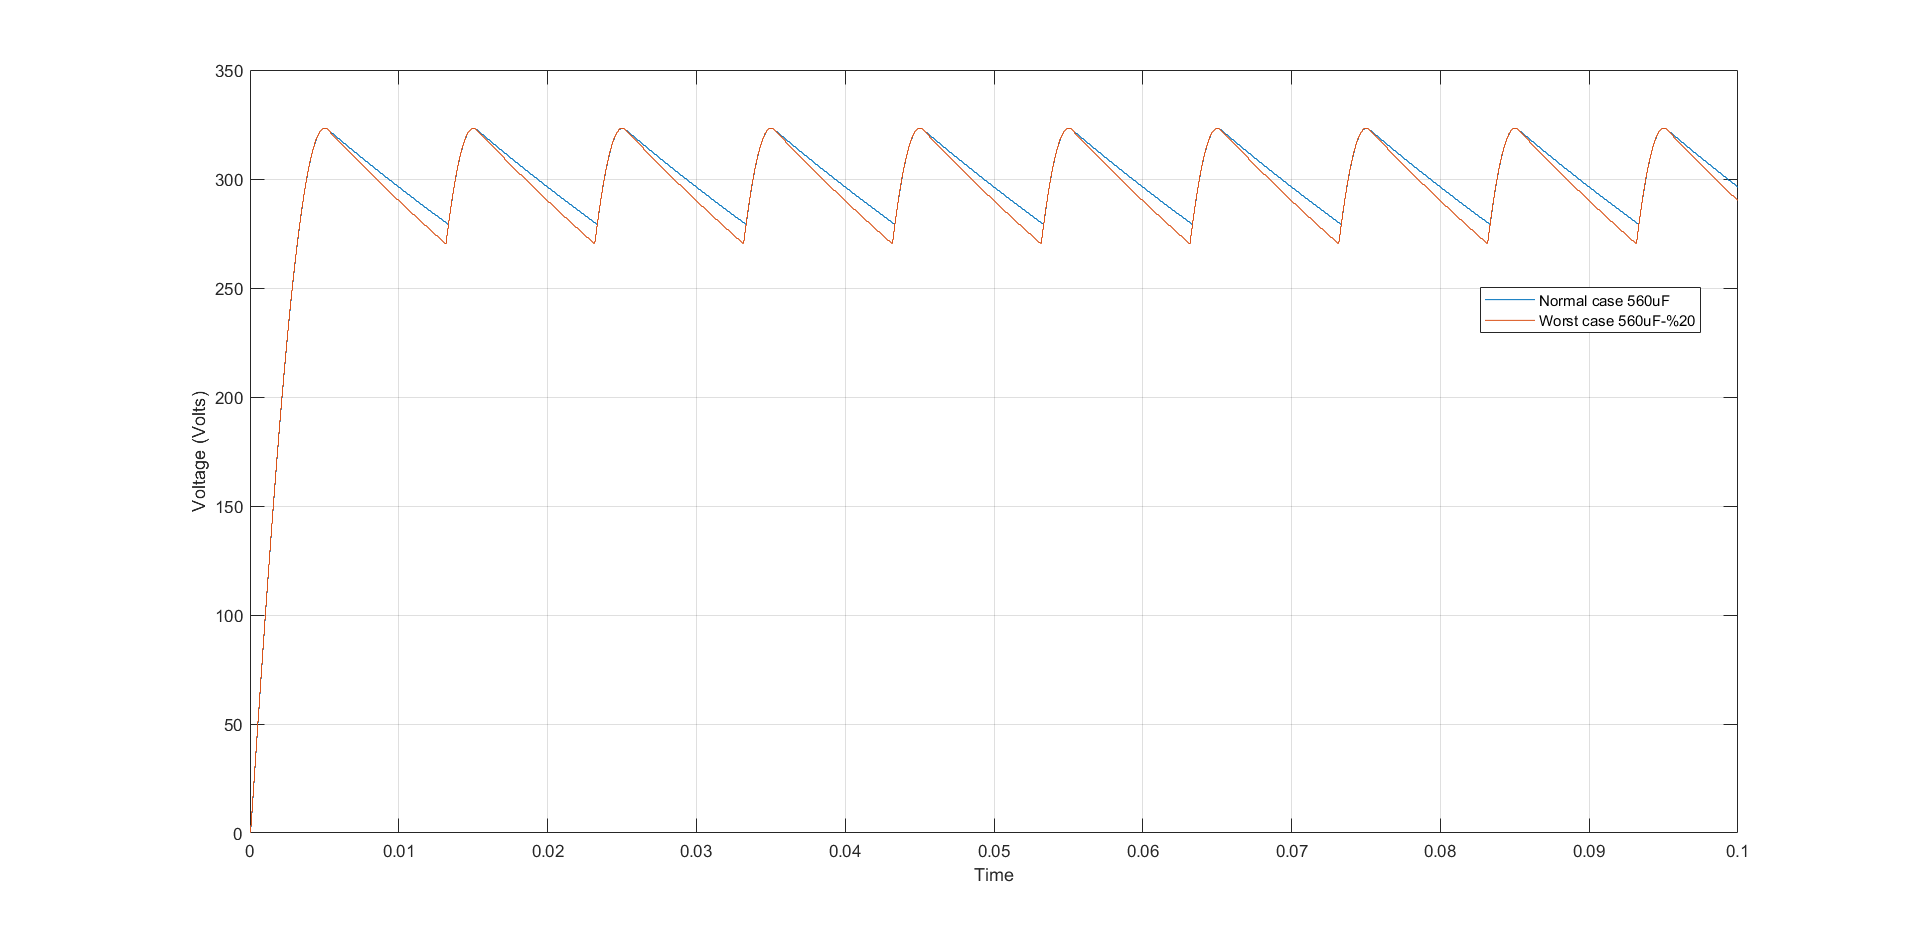
\includegraphics[width=\linewidth]{RC_load.png}
  \caption{Output waveforms both worst case and normal case scenario with RC load.}
  \label{fig:simulink2}
\end{figure}
Our ripple current (low frequency) is about 0.5 A range therefore our capacitance satisfy our ripple current requirement as well. 

\begin{figure}[H]
  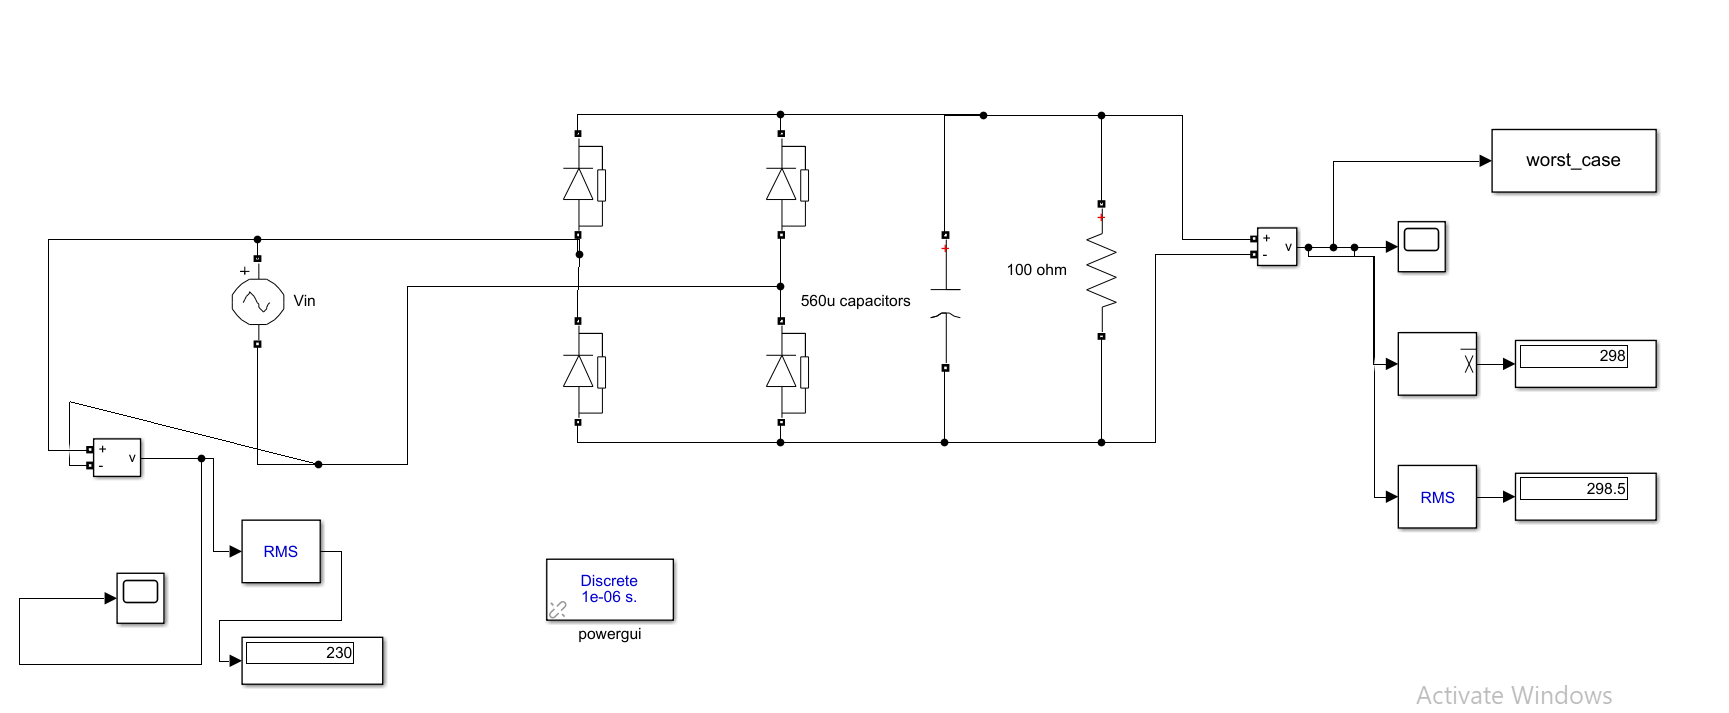
\includegraphics[width=\linewidth]{Simulink_modelRC_load.PNG}
  \caption{Simulink model of the full bridge rectifier}
  \label{fig:simulink3}
\end{figure}
Ripple voltages (both worst and normal cases) are given in following table;

\begin{table}[H]
\centering
\begin{tabular}{lll}
                       & Worst case & Normal case \\
Average output voltage & 298 V      & 302.2 V     \\
Ripple Voltage         & 53.6 V     & 44.3 V      \\
Ripple ratio           & \%18       & \%14.63    
\end{tabular}
\caption{Ripple analysis with normal and worst case scenarios}
\end{table}
\subsection*{Part 4}
At this part we observed the effect of line inductance at the source side. Since inductor current is continuous we observed \textbf{smoother current waveform} (less crest factor) with added line inductance. The output ripple voltage does not change much only the frequency increased at steady state. The effect of line inductance is mostly seen \textit{transient} output voltage. 
\begin{figure}[H]
  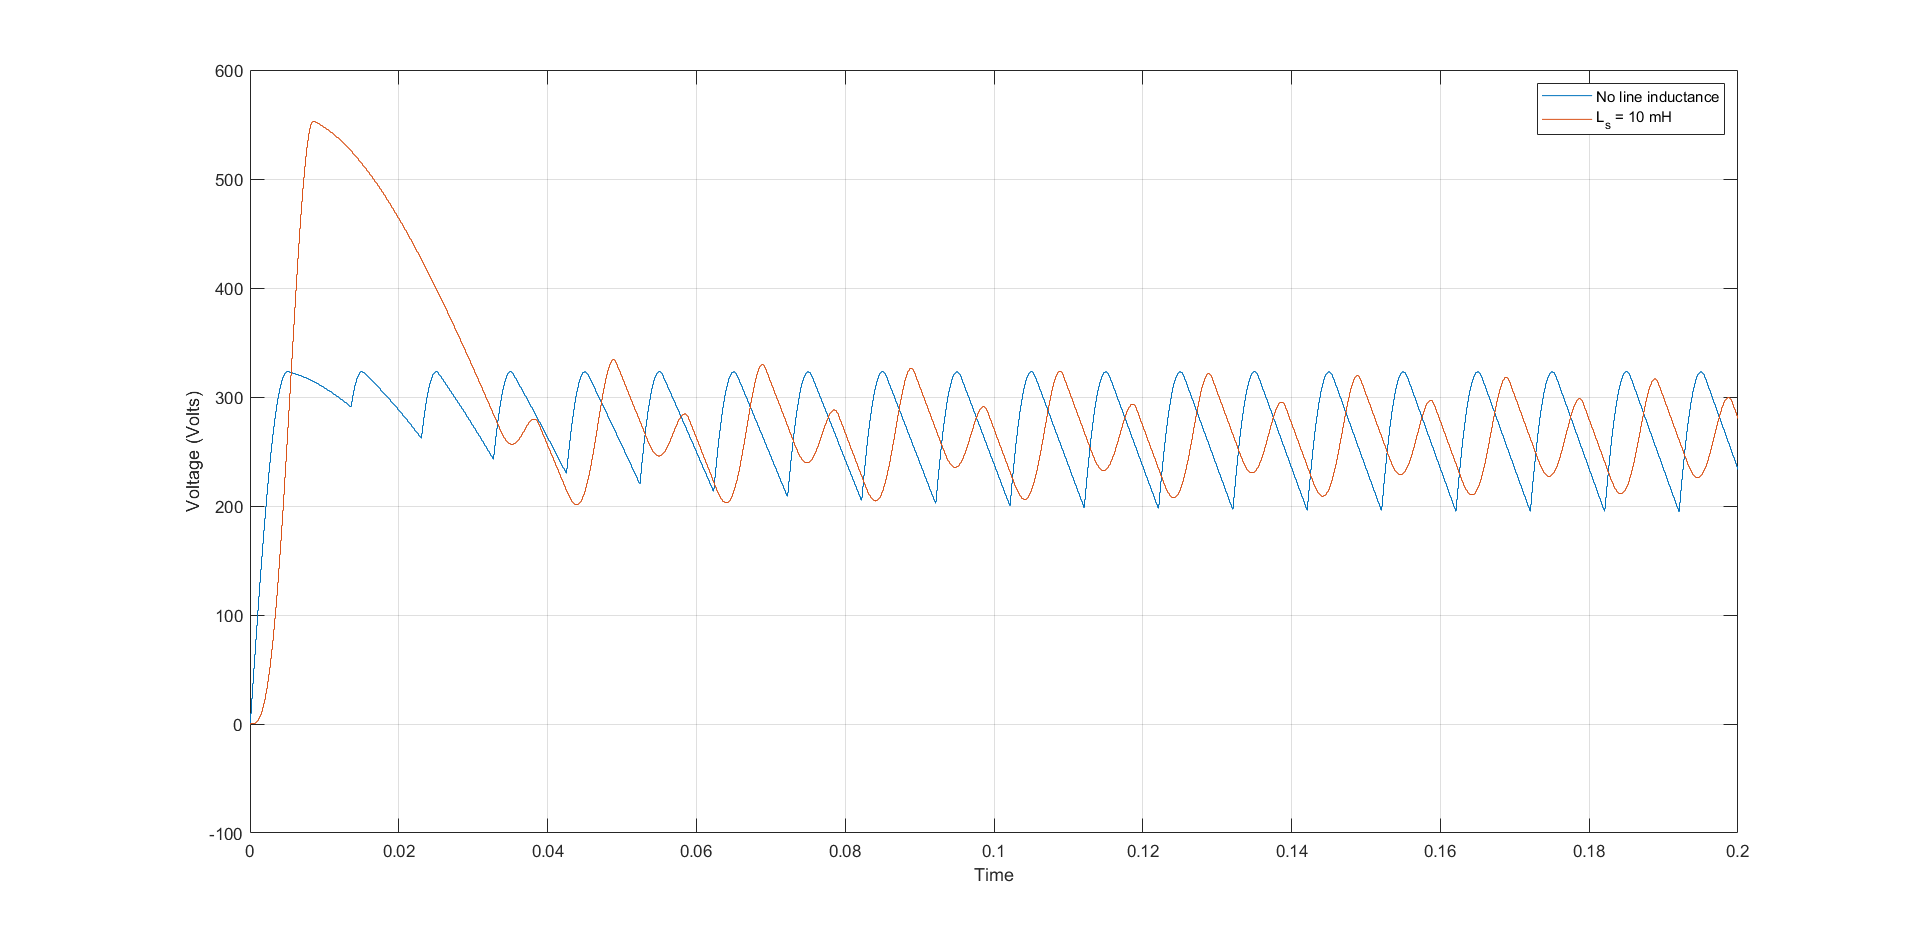
\includegraphics[width=\linewidth]{part2d.png}
  \caption{The effect of line inductance on output voltage waveform}
  \label{fig:simulink3}
\end{figure}
\begin{figure}[H]
  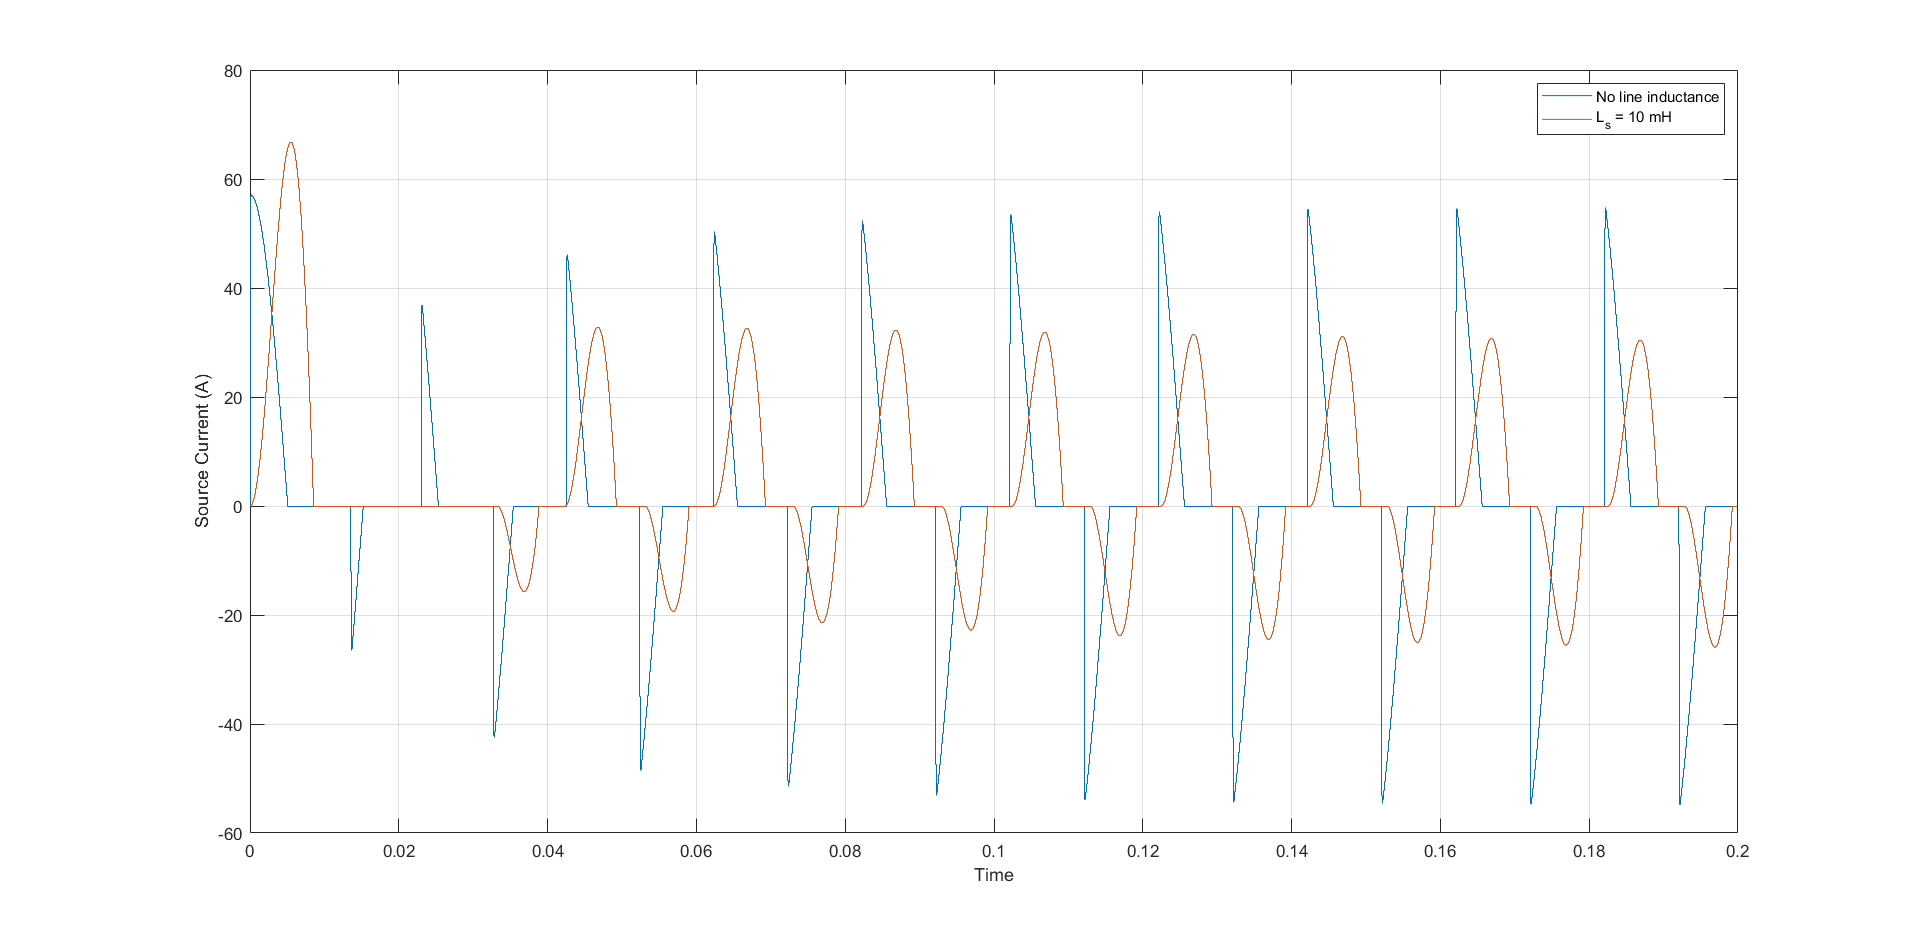
\includegraphics[width=\linewidth]{part2d2.png}
  \caption{The effect of line inductance on source current}
  \label{fig:simulink3}
\end{figure}
\subsection*{Part 5}

In this section, we have observed how voltage is seen from another equipment at the point of common coupling. Since current drawn by rectifier diodes undergo a distortion due to the nonlinear load (in this case diode rectifier), that distortion concludes with a distortion in voltage waveform.As can be seen in Figure 10, voltage waveform of source and voltage waveform of point of common coupling has slight difference due to distortion. 

\begin{figure}[H]
  \includegraphics[width=\linewidth]{part25.png}
  \caption{Voltage Waveforms of Source, Point of Common Coupling and Load}
  \label{fig:simulink3}
\end{figure}


\section*{Question 3}
In this part we have simulated three-phase diode bridge rectifier and observed power factor, THD of output current and waveforms of neutral, phase current and output voltage.
\subsection*{Part 1}
\begin{figure}[H]%
    \centering
    \subfloat[R=25 ohm]{{\includegraphics[width=7cm]{thd2.png}}}%
    \qquad
    \subfloat[R=25 ohm L = 10 mH]{{\includegraphics[width=7cm]{thd1.png} }}%
    \caption{FFT analysis with line inductance (left) and without line inductance (right)}%
    \label{fig:example}%
\end{figure}
\begin{figure}[H]
  \includegraphics[width=\linewidth]{currents31.png}
  \caption{Phase and Neutral line currents}
  \label{fig:simulink3}
\end{figure}

\begin{figure}[H]
  \includegraphics[width=\linewidth]{outputvoltage31.png}
  \caption{Load voltage at steady state}
  \label{fig:simulink3}
\end{figure}
\subsection*{Part 2}

In three-phase rectifiers each phase becomes dominant only 120 degree in each period. Since neutral line which transmits sum of the all phase currents, frequency of the neutral line current becomes three times of the grid frequency which is 50 Hz. The reason which makes neutral line current bigger than phase current is phase current's becoming 0 for 120 degree while neutral current is never 0.
\subsection*{Part 3}
\begin{figure}[H]
  \includegraphics[width=\linewidth]{outputvoltage33.png}
  \caption{The effect of line inductance on output voltage}
  \label{fig:simulink3}
\end{figure}
\begin{figure}[H]
  \includegraphics[width=\linewidth]{neutralcurrent33.png}
  \caption{The effect of line inductance on neutral wire current}
  \label{fig:simulink3}
\end{figure}
\begin{figure}[H]
  \includegraphics[width=\linewidth]{phase_currents33.png}
  \caption{The effect of line inductance on phase A current}
  \label{fig:simulink3}
\end{figure}
\end{document}
